\documentclass[../main.tex]{subfiles}

% \title{Abbe sine condition}
% \date{2018-02-05}
% \author{Hongjie Lu}

\begin{document}

	% \maketitle
	% \pagenumbering{gobble}
	% \newpage
	\section{History of Diffraction theory}
	\begin{figure}[h!]
	  \centering
	  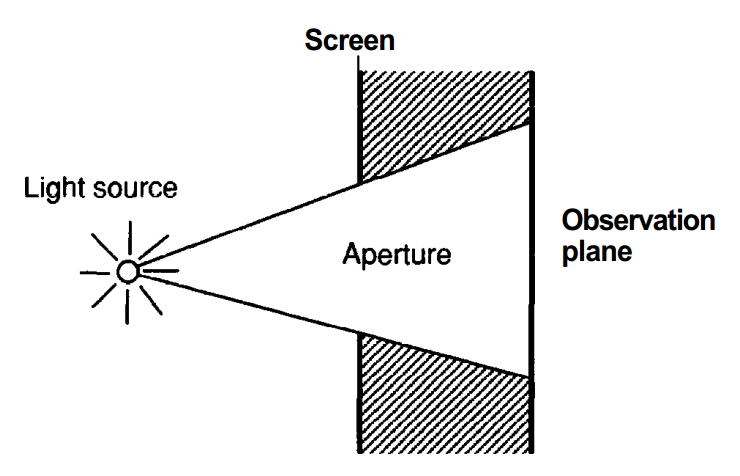
\includegraphics[scale=0.5]{../graphics/Wave_optics1.png}
	  \caption{Grimaldi's observations}
	  \label{fig:Grimaldi}
	\end{figure}
	1665, Grimaldi's observations showed the shadow behind the opaque screen with a aperture was not with sharp borders but with gradual transition. This phenomenon can not be explained by the corpuscular theory of light propagation.\ref{fig:Grimaldi}

	\begin{figure}[h!]
	  \centering
	  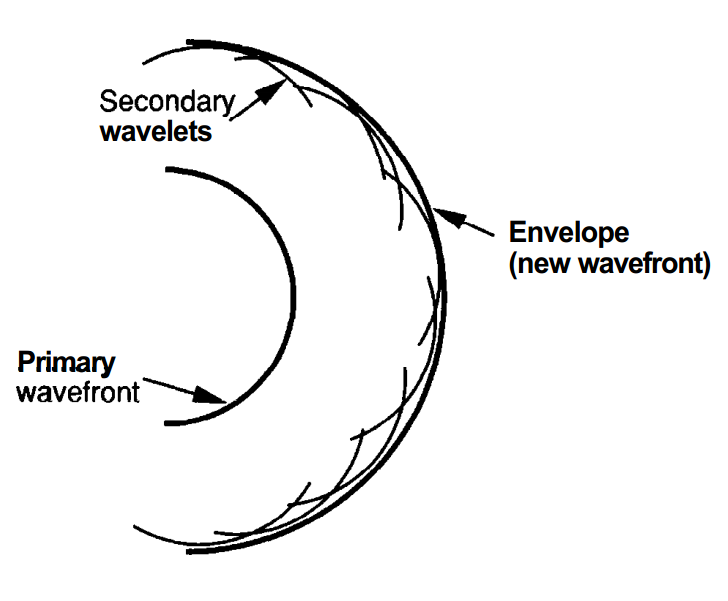
\includegraphics[scale=0.5]{../graphics/Wave_optics2.png}
	  \caption{Huygens' envelope construction}
	  \label{fig:Huygens}
	\end{figure}

	1678, Huygens expressed the intuitive conviction that if each point on the wavefront of a disturbance were considered to be a new source of a "secondary" spherical disturbance, then the wavefront at a later instant could be found by constructing the "envelope" of the secondary wavelets.\ref{fig:Huygens}

	1804, Thomas Young strengthen the wave theory of light by introducing the critical concept of interference. The idea was a radical one at the time, for it stated that under proper conditions, light could be added to light and produce darkness.

	1818, Augustion Jean Fresnel brought together the ideas of Huygens and Young. By making some rather arbitary assumptions about the amplitudes and phases of Huygens' secondary sources, and by allowing the various wavelets to mutually interfere, Fresnel was able to calculate the distribution of light in diffraction patterns with excellent accuracy. 

	At Fresnel's presentation of his paper to a prize committee of the French Academy of Sciences, his theory was strongly disputed by the great French mathematician S. Poisson, a member of the committee. He demonstrated the absurdity of the theory by showing that it predicted the existence of a bright spot at the center of the shadow of an opaque disk. F. Arago, who chaired the prize committee, performed such an experiment and found the predicted spot. Fresnel won the prize, and since then the effect has been known as "Poisson's spot".

	1860, Maxwell identified light as an electronmagnetic wave, a step of enormous importance.

	1882, Gustav Kirchhoff put the ideas of Huygens and Fresnel on a firmer mathematical foundation with two assumptions about the boundary values of the light incident on the surface of an obstacle placed in the way of propagation of light. These assumptions were later proved to be inconsistent with each other, by PoincarC in 1892 and by Sommerfeld in 1894.' As a consequence of these criticisms, Kirchhoff's formulation of the so-called Huygens-Fresnel principle must be regarded as a first approximation, although under most conditions it yields results that agree amazingly well with experiment. 

	Sommerfeld modified the Kichhoff theory by eliminating one of the assumptions concerning the light amplitude at the boundary by making use of the theory of Green's functions. This is called Rayleigh-Sommerfeld diffraction theory.

	The Kirchhoff and Rayleigh-Sommerfeld theories share certain major simplifications and approximations thta light is treated as scalar phenomenon, neglecting the fundamentally vectorial nature of the electromagnetic fields. The scalar theory yields very accurate results if two conditions are met: (1) the diffracting aperture must be large compared with a wavelength, and (2) the diffracting fields must not be observed too close to the aperture. 

	\section{From a vector to a scalar theory}

	Maxwell's equations:
	\begin{align}
	&\boldsymbol{\bigtriangledown}\times\vec{\varepsilon}=-\mu\frac{\delta \vec{H}}{\delta t}\\
	&\boldsymbol{\bigtriangledown}\times\vec{H}=\epsilon\frac{\delta \vec{\varepsilon}}{\delta t}\\
	&\boldsymbol{\bigtriangledown}\cdot\epsilon\vec{\varepsilon}=0\\
	&\boldsymbol{\bigtriangledown}\cdot\mu\vec{H}=0
	\end{align}

	Here $\vec{\varepsilon}$ is the electric field, with rectilinear components $(\vec{\varepsilon}_{X},\vec{\varepsilon}_{Y},\vec{\varepsilon}_{Z})$, and $\vec{H}$ is the magnetic field, with components $(\vec{H}_{X},\vec{H}_{Y},\vec{H}_{Z})$. $\vec{\varepsilon}$ and $\vec{H}$ are functions of both position P and time t. The symbols $\times$ and $\cdot$ represent a vector cross product and a vector dot product respectively, while $\boldsymbol{\bigtriangledown}=\frac{\delta \vec{i}}{\delta x}+\frac{\delta \vec{j}}{\delta y}+\frac{\delta \vec{k}}{\delta z}$, where $\vec{i},\vec{j},\vec{k}$ are unit vector in the x, y z directions respectively.

	Assumption:
	\begin{itemize}
  	\item The wave is propagating in a dielectric medium.
  	\item The medium is linear if it satisfies the linearity properties.
  	\item The medium is isotropic if its properties are independent of the direction of polarization of the wave.
  	\item The medium is homogeneous if the permittivity is constant throughout the region of propagation.
  	\item The medium is nondispersive if the permittivity is independent of wavelength over the wavelength region occupied by the propagating wave.
  	\item The medium is nonmagnetic, the magnetic permeability is always equal to po, the vacuum permeability.
	\end{itemize}

	Applying the $\boldsymbol{\bigtriangledown}\times$ operation to the left and right sides of the first equation for $\vec{\varepsilon}$, and make use of Vector calculus identities, we can get
	\begin{equation}
	\boldsymbol{\bigtriangledown}\times(\boldsymbol{\bigtriangledown}\times\vec{\varepsilon})=\boldsymbol{\bigtriangledown}(\boldsymbol{\bigtriangledown}\cdot\vec{\varepsilon})-\boldsymbol{\bigtriangledown}^2\vec{\varepsilon}
	\end{equation}
	If the propagation medium is linear, isotropic, homogeneous, and nondispersive, we can get
	\begin{equation}
	\boldsymbol{\bigtriangledown}^2\vec{\varepsilon}-\frac{n^2}{c^2}\frac{\delta^2 \vec{\varepsilon}}{\delta t^2}=0
	\end{equation}
	where n is the refractive index of the medium and c is the velocity of propagation in vacuum.

	The same for magnetic field:
	\begin{equation}
	\boldsymbol{\bigtriangledown}^2\vec{H}-\frac{n^2}{c^2}\frac{\delta^2 \vec{H}}{\delta t^2}=0
	\end{equation}

	Since the vector wave equation is obeyed by both $\vec{\varepsilon}$ and $\vec{H}$, an identical scalar wave equation is obeyed by all components of those vectors, for example:
	\begin{equation}
	\boldsymbol{\bigtriangledown}^2\vec{\varepsilon}_X-\frac{n^2}{c^2}\frac{\delta^2 \vec{\varepsilon}_X}{\delta t^2}=0
	\end{equation}
	To summarize, the behavior of all components of $\vec{\varepsilon}$ and $\vec{H}$ through a single scalar wave equation:
	\begin{equation}
	\boldsymbol{\bigtriangledown}^2u(P,t)-\frac{n^2}{c^2}\frac{\delta^2 u(P,t)}{\delta t^2}=0
	\label{eq2-1}
	\end{equation}
	where $u(P,t)$ represents any of the scalar field components dependent on position P in space and time t.

	\section{Kirchhoff diffraction}
	\subsection{The Helmholtz Equation}
	Only monochromatic wave considered here, the scalar field for monochromatic wave is 
	\begin{equation}
	u(P,t)=A(P)\cos{[2\pi vt+\phi(P)]}
	\end{equation}
	where A(P) and $\phi(P)$ are the amplitude and phase of the wave at position P, while v is the optical frequency. The equation can be formed in complex notation:
	\begin{equation}
	u(P,t)=Re{\{U(P)exp(-j2\pi vt)\}}
	\end{equation}
	where $Re{\{\}}$ signifies "real part of", and U(P) is a complex function of position (sometimes called a phasor)
	\begin{equation}
	U(P)=A(P)exp[-j\phi(P)]
	\end{equation}
	according to equation \ref{eq2-1}, we can get 
	\begin{equation}
	(\boldsymbol{\bigtriangledown}^2+k^2)U=0
	\label{eq3-1}
	\end{equation}
	here k is termed the wave number and is given by
	\begin{equation}
	k=2\pi n \frac{v}{c}=\frac{2\pi}{\lambda}
	\end{equation}
	The equation \ref{eq3-1} is known as the Helmholtz equation

	\subsection{Green's theorem}
	Let U(P) and G(P) be any two complex-valued functions of position, and let S be a closed surface surrounding a colume V. If U, G, and their first and second partial derivatives are single-valued and continuous within and on S, then we have
	\begin{equation}
	\iiint_V (U\boldsymbol{\bigtriangledown}^2G-G\boldsymbol{\bigtriangledown}^2U)dv=\iint_S (U\frac{\delta G}{\delta n}-G\frac{\delta U}{\delta n})ds
	\end{equation}

	\subsection{The integral theorem of Helmholtz and Kirchhoff}
	Let the point of observation be denoted $P_0$, and let S denote an arbitary closed surface surrounding $P_0$. The problem is to express the optical disturbance at $P_0$ in terms of its values on the surface S. To solve this problem, we follow Korchhoff in applying Green's theorem and in choosing as an auxiliary function a unit-amplitude spherical wave expanding about the point $P_0$ ( the so-called free space Green's function). Thus the value of Kirchhoff's G at an arbitary point $P_1$ is given by 
	\begin{equation}
	G(P_1)=\frac{exp(jkr_{01})}{r_{01}}
	\end{equation}
	where we adopt the notation that $r_{01}$ is the length of the vector $\vec{r_{01}}$ pointing from $P_0$ to $P_1$

	...

	To be legitimately used in Green's theorem, the function G must be continuous within the enclosed volume V. Therefore to exclude the discontinuity at $P_0$, a small spherical surface $S_\epsilon$ of radius $\epsilon$ is inserted about the point $P_0$. Green's theorem is then applied, the volume of integration V' being that volume lying between S and $S_\epsilon$, and the surface of integration being the composite surface
	\begin{equation}
	S'=S+S_\epsilon
	\end{equation}

	as indicated in fig \ref{fig:integration}. Note that the outward normal normal to the composite surface points outward in the conventional sense on S, but inward(towards $P_0$) on $S_\epsilon$

	\begin{figure}[h!]
	  \centering
	  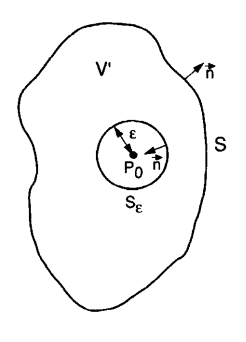
\includegraphics[scale=0.5]{../graphics/Wave_optics3.png}
	  \caption{Surface of integration.}
	  \label{fig:integration}
	\end{figure}

	Within the volume V', the disturbance G being simply an expanding spherical wave, satisfies the Helmholtz equation
	\begin{equation}
	(\boldsymbol{\bigtriangledown}^2+k^2)G=0
	\label{eq3-1}
	\end{equation}

	Substituting the equation in the left-hand side of Green's theorem, we find
	\begin{equation}
	\iiint_{V'} (U\boldsymbol{\bigtriangledown}^2G-G\boldsymbol{\bigtriangledown}^2U)dv=-\iiint_{V'} (UGk^2-GUk^2)dv\equiv0
	\end{equation}
	Thus the theorem reduces to 
	\begin{align}
	\iint_{S'} (U\frac{\delta G}{\delta n}-G\frac{\delta U}{\delta n})ds=0\\
	-\iint_{S_\epsilon} (U\frac{\delta G}{\delta n}-G\frac{\delta U}{\delta n})ds=\iint_{S} (U\frac{\delta G}{\delta n}-G\frac{\delta U}{\delta n})ds
	\end{align}

	Note for a general point $P_1$ on S', we have
	\begin{align}
	G(P_1)=\frac{exp(jkr_{01})}{r_{01}}\\
	\frac{\delta G(P_1)}{\delta n}=\cos(\vec{n},\vec{r}_{01})(jk-\frac{1}{r_{01}})\frac{exp(jkr_{01})}{r_{01}}
	\end{align}
	where $\cos(\vec{n},\vec{r_{01}})$ represents the cosine of the angle between the outward normal $\vec{n}$ and the vector $\vec{r_{01}}$ joining $P_0$ to $P_1$. For the particular case of $P_1$ on $S_\epsilon$, $\cos(\vec{n},\vec{r_{01}})=-1$, and the equations become
	\begin{align}
	G(P_1)=\frac{exp(jk\epsilon)}{\epsilon}\\
	\frac{\delta G(P_1)}{\delta n}=\frac{exp(jk\epsilon)}{\epsilon}(\frac{1}{\epsilon}-jk)
	\end{align}

	Letting $\epsilon$ become arbitarily small, the continuity of U and its derivatives at $P_0$ allows us to write
	\begin{align}
	\lim_{\epsilon\to 0}{\iint_{S_\epsilon}\left(U\frac{\delta G}{\delta n}-G\frac{\delta U}{\delta n}\right)}ds
	=\lim_{\epsilon\to 0}4\pi\epsilon^2\left[U(P_0)\frac{exp(jk\epsilon)}{\epsilon}\left(\frac{1}{\epsilon}-jk\right)-\frac{\delta U(P_0)}{\delta n}\frac{exp(jk\epsilon)}{\epsilon}\right]
	=4\pi U(P_0)
	\end{align}

	\begin{equation}
	U(P_0)=\frac{1}{4\pi}\iint_S\left\{\frac{\delta U}{\delta n}\left[\frac{exp(jkr_{01})}{r_{01}}\right]-U\frac{\delta}{\delta n}\left[\frac{exp(jkr_{01})}{r_{01}}\right]\right\}ds
	\end{equation}

	This result is known as the integral theorem of Helmholtz and Kirchhoff. It plays an important role in the development of the scalar theory of diffraction, for it allows the field at any point $P_0$ to be expressed in terms of the boundary values of the wave on any closed surface surrounding that point.

	\subsection{Kirchhoff diffraction by a planar screen}
	Consider now the problem of diffraction of light by an aperture in an infinite opaque screen. As illustrated in Fig \ref{fig:Kirchhoff}, a wave disturbance is assumed to impinge on the screen and the aperture from the left, and the field at the point Pobehind the aperture is to be calculated. Again the field is assumed to be monochromatic.

	\begin{figure}[h!]
	  \centering
	  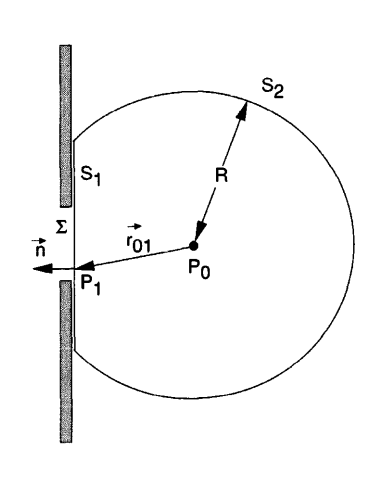
\includegraphics[scale=0.5]{../graphics/Wave_optics4.png}
	  \caption{Kirchhoff formulation of diffraction by a plane screen}
	  \label{fig:Kirchhoff}
	\end{figure}

	Following Kirchhoff, the closed surface S is chosen to consist of two parts, as shown in Fig \ref{fig:Kirchhoff}. Let a plane surface $S_1$, lying directly behind the diffracting screen, be joined and closed by a large spherical cap, $S_2$, of radius R and centered at the observation point $P_0$. The total closed surface S is simply the sum of $S_1$ and $S_2$. Thus, 
	\begin{equation}
	U(P_0)=\frac{1}{4\pi}\iint_{S_1+S_2}\left(G\frac{\delta U}{\delta n}-U\frac{\delta G}{\delta n}\right)ds
	\end{equation}
	...
	It can be proved that the integral over $S_2$ will yield a contribution pf zero so we can have 
	\begin{equation}
	U(P_0)=\frac{1}{4\pi}\iint_{S_1}\left(G\frac{\delta U}{\delta n}-U\frac{\delta G}{\delta n}\right)ds
	\end{equation}

	For the opaque screen with open aperture denoted as $\Sigma$, it therefore seems intuitively reasonable that the major contribution to the integral arises from the points of $S_1$ located within the aperture $\Sigma$ where we would expect the integrand to be largest. Kirchhoff accordingly adopted the following assumptions:
	\begin{itemize}
	\item Across the surface $\Sigma$ the field distribution U and its derivative $\frac{\delta U}{\delta n}$ are exactly the same as they would be in the absence of the screen.\\
	\item Over the portion of $S_1$ that lies in the geometrical shadow of the screen, the field distribution U and its derivative $\frac{\delta U}{\delta n}$ are identically zero
	\end{itemize}

	These conditions are commonly known as the Kirchhoff boundary conditions. The first allows us to specify the disturbance incident on the aperture by neglecting the presence of the screen. The second allows us to neglect all of the surface of integration except that portion lying directly within the aperture itself.

	And the equation can be reduced to
	\begin{equation}
	U(P_0)=\frac{1}{4\pi}\iint_{\Sigma}\left(G\frac{\delta U}{\delta n}-U\frac{\delta G}{\delta n}\right)ds
	\end{equation}

	While the Kirchhoff boundary conditions simplify the results considerably, it is important to realize that neither can be exactly true. The presence of the screen will inevitably perturb the field on $\Sigma$ to some degree, for along the rim of the aperture certain boundary condition must be met that would not be required in the absence of the screen. In addition, the shadow behind the screen is never perfect, for fields will inevitably extend behind the screen for a distance of several wavelengths. However, if the dimensions of the aperture are large compared with a wavelength, these fringing effects can be safely neglected, and the two boundary conditions can be used to yield results that agree very well with experiment.

	\subsection{The Fresnel-Kirchhoff diffraction formula}
	A further simplification of the expression for $U(P_0)$ is obtained by noting that the distance $r_{01}$ from the aperture to the observation point is usually many optical wavelengths; and if we made the same assumption for the point source $P_2$ and the distance $r_{21}$ from $P_1$ we have
	\begin{align}
	k\gg\frac{1}{r_{01}}\\
	k\gg\frac{1}{r_{02}}\\
	\frac{\delta G(P_1)}{\delta n}=\cos(\vec{n},\vec{r}_{01})(jk-\frac{1}{r_{01}})\frac{exp(jkr_{01})}{r_{01}}\approx jk \cos(\vec{n},\vec{r}_{01})\frac{exp(jkr_{01})}{r_{01}}\\
	U(P_1)=\frac{A exp(jkr_{21})}{r_{21}}\\
	\frac{\delta U(P_1)}{\delta n}=A\cos(\vec{n},\vec{r}_{21})(jk-\frac{1}{r_{21}})\frac{exp(jkr_{21})}{r_{21}}\approx Ajk \cos(\vec{n},\vec{r}_{21})\frac{exp(jkr_{21})}{r_{21}}
	\end{align}
	\begin{multline}
	U(P_0)=\frac{1}{4\pi}\iint_\Sigma\left\{\frac{\delta U}{\delta n}\left[\frac{exp(jkr_{01})}{r_{01}}\right]-U\frac{\delta}{\delta n}\left[\frac{exp(jkr_{01})}{r_{01}}\right]\right\}ds\\
	=\frac{1}{4\pi}\iint_\Sigma\frac{exp(jkr_{01})}{r_{01}}\left[\frac{\delta U}{\delta n}-jkU\cos(\vec{n},\vec{r_{01}})\right]ds\\
	=\frac{A}{j\lambda}\iint_\Sigma{\frac{exp(jk(r_{01}+r_{02})}{r_{01}r_{02}}}\left[\frac{\cos(\vec{n},\vec{r_{01}})-\cos(\vec{n},\vec{r_{21}})}{2}\right]ds
	\end{multline}

	This result is known as the Fresnel-Kirchhoff diffraction formula. This equation can be written in another form:
	\begin{equation}
	U(P_0)=\iint_\Sigma{U'(P_1)\frac{exp(jkr_{01})}{r_{01}}}ds
	\end{equation}
	where
	\begin{equation}
	U'(P_1)=\frac{1}{j\lambda}\left[\frac{A exp(jkr_{21}}{r_{21}}\right]\left[\frac{\cos(\vec{n},\vec{r_{01}})-\cos(\vec{n},\vec{r_{21}})}{2}\right]
	\end{equation}

	This equaiton may be interpreted as implying that the field at $P_0$ arises from an infinity of fictitious secondary point sources located within the aperture itself.

	Note that the above derivation has been restricted to the case of an aperture illumination consisting of a single expanding spherical wave. However, such a limitation can be removed by the Rayleigh-Sommerfeld theory.

	\subsection{Rayleigh-Sommerfeld theory}
	First Rayleigh-Sommerfeld solution:
	\begin{align}
	G_-(P_1)=\frac{exp(jkr_{01})}{r_{01}}-\frac{exp(jk\tilde{r}_{01})}{\tilde{r}_{01}}\\
	U_I(P_0)=\frac{-1}{4\pi}\iint_\Sigma{U\frac{\delta G_-}{\delta n}}ds=\frac{-1}{2\pi}\iint_\Sigma{U\frac{\delta G}{\delta n}}ds=\frac{1}{j\lambda}\iint_{\Sigma} U(P_1)\frac{exp(jkr_{01})}{r_{01}}\cos(\vec{n},\vec{r}_{01})ds\label{first R-S solution}
	\end{align}
	Second Rayleigh-Sommerfeld solution:
	\begin{align}
	G_+(P_1)=\frac{exp(jkr_{01})}{r_{01}}+\frac{exp(jk\tilde{r}_{01})}{\tilde{r}_{01}}\\
	U_{II}(P_0)=\frac{1}{4\pi}\iint_\Sigma{\frac{\delta U}{\delta n}}G_+ds=\frac{1}{2\pi}\iint_\Sigma{\frac{\delta U}{\delta n}}Gds=\frac{1}{2\pi}\iint_\Sigma{\frac{\delta U(P_1)}{\delta n}}\frac{exp(jkr_{01})}{r_{01}}ds
	\end{align}
	
	\section{Fresnel and Fraunhofer Diffraction}
	\subsection{The intensity of a wave field}
	\subsection{The Huygens-Fresnel Principle in Rectangular Coordinates}
	\begin{figure}[h!]
	  \centering
	  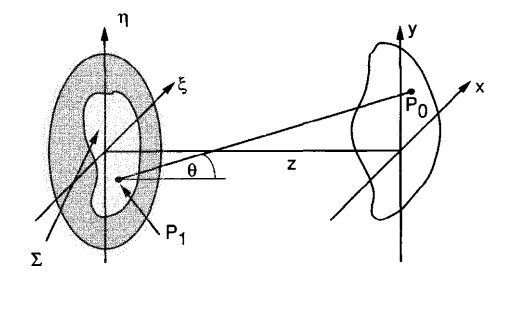
\includegraphics[scale=0.5]{../graphics/Wave_optics5.png}
	  \caption{Diffraction geometry}
	  \label{fig:Coordinates}
	\end{figure}
	First state the principle in more explicit form for the case of rectangular coordinates. As shown in fig \ref{fig:Coordinates}, the diffraction aperture is assumed to lie in the left plane and is illuminated in the positive z direction. We will calculate the wavefield across the (x,y) plane, which is parallel to the aperture plane.

	According to First Rayleigh-Sommerfeld solution equation \ref{first R-S solution}, the Huygens-Fresnel principle can be stated as
	\begin{equation}
	U(P_0)=\frac{1}{j\lambda}\iint_{\Sigma} U(P_1)\frac{exp(jkr_{01})}{r_{01}}\cos(\theta)ds
	\end{equation}
	where $\theta$ is the angle between the outward normal and the vector pointing from $P_0$ to $P_1$. The term $cos\theta$ is given exactly by
	\begin{equation}
	\cos\theta=\frac{z}{r_{01}}
	\end{equation}
	Therefore we can rewrite the equation:
	\begin{equation}
	U(x,y)=\frac{z}{j\lambda}\iint_{\Sigma} U(\xi,\eta)\frac{exp(jkr_{01})}{r^2_{01}}d\xi d\eta\label{Fresnel}
	\end{equation}
	where the distance $r_{01}$ is given by
	\begin{equation}
	r_{01}=\sqrt{z^2+(x-\xi)^2+(y-\eta)^2}
	\end{equation}

	There have been only two approximations inreaching this expression. One is the approximation inherent in the scalar theory. The second is the assumption that the observation distance is many wavelangths from the aperture, $r_{01}\gg\lambda$.
	\subsection{Fresnel Diffraction}
	To reduce the Huygens-Fresnel principle to a more simple and usable expression, we introduce approximations for the distance $r_{01}$ between $P_1$ and $P_0$. 
	\begin{equation}
	\sqrt{1+b}=1+\frac{1}{2}b-\frac{1}{8}b^2+...
	\end{equation}
	where the number of terms needed for a given accuracy depends on the magnitude of b. Apply this binomial expansion to the $r_{01}$, we can get
	\begin{equation}
	r_{01}=z\sqrt{1+\left(\frac{x-\xi}{z}\right)^2+\left(\frac{y-\eta}{z}\right)^2}\approx z\left[1+\frac{1}{2}\left(\frac{x-\xi}{z}\right)^2+\frac{1}{2}\left(\frac{y-\eta}{z}\right)^2\right]
	\end{equation}
	The question now arises as to whether we need to retain all the terms in the approximation, or whether only the first term might suffice. The answer to this question depends on which of the several occurrences of $r_{01}$ is being approximated. 
	\begin{itemize}
	\item for the $r^2_{01}$ in the denominator of equation \ref{Fresnel}, the error introduced by dropping all terms but z is generally acceptably small.
	\item for $r_{01}$ appearing in the exponent, errors are much more critical. First, they are multiplied by a very large number k. Second, phase changes of as little as a fraction of a radian can change the value of the exponential significantly. For this reason we retain both terms of the binomial approximation in the exponent.
	\end{itemize}
	The resulting expression for the field at (x,y) of equation \ref{Fresnel} becomes:
	\begin{equation}
	U(x,y)=\frac{exp(jkz)}{j\lambda z}\iint_{-\infty}^{+\infty} U(\xi,\eta)exp\left\{j\frac{k}{2z}\left[(x-\xi)^2+(y-\eta)^2\right]\right\}d\xi d\eta\label{Fresnel2}
	\end{equation}
	where we have incorporated the finite limits of the aperture in the definition of $U(\xi,\eta)$, in accord with the usual assumed boundary conditions.

	This equation \ref{Fresnel2} can be seen be to a convolution, expressible in the form
	\begin{align}
	U(x,y)=\iint_{-\infty}^{+\infty} U(\xi,\eta)h(x-\xi,y-\eta)d\xi d\eta\label{convolution}\\
	h(x,y)=\frac{exp(jkz)}{j\lambda z}exp\left[\frac{jk}{2z}(x^2+y^2)\right]\label{quadratic-phase}
	\end{align}

	Another form the the equation \ref{Fresnel2} is Fourier transform of the product of the complex field just to the right of the aperture and a quadratic phase exponential.
	\begin{equation}
	U(x,y)=\frac{exp(jkz)}{j\lambda z}exp\left[\frac{jk}{2z}(x^2+y^2)\right]\iint_{-\infty}^{+\infty} \left\{U(\xi,\eta)exp\left[\frac{jk}{2z}(\xi^2+\eta^2)\right]\right\}exp\left[-j\frac{2\pi}{\lambda z}(x\xi+y\eta)\right]d\xi d\eta\label{Fourierform}
	\end{equation}
	We refer to both forms of the results as the Fresnel diffraction integral. When this approximation is valid, the observer is said to be in the region of Fresnel diffraction, or equivalently in the near field of the aperture.

	\subsection{Positive or negative phases}
	It is common practice when using the Fresnel approximation to replace expressions for spherical waves by quadratic-phase exponentials. The question often arises as to whether the sign of the phase should be positive or negative in a given expression.

	The critical fact to keep in mind is that we have chosen our phasors to rotate in the clockwise direction, i.e. their time dependence is of the form $exp(-j2\pi vt)$. For this reason, if we move in space in such a way as to intercept portions of a wavefield that were emitted later in time, the phasor will have advanced in the clockwise irection, and therefore the phase must become more negative. 

	\begin{figure}[h!]
	  \centering
	  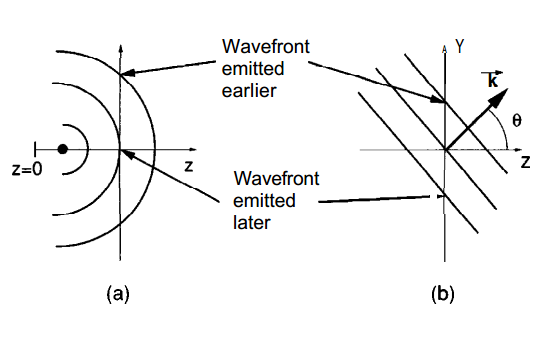
\includegraphics[scale=0.5]{../graphics/Wave_optics6.png}
	  \caption{Determining the sign of the phases of exponential representations of spherical/plane waves}
	  \label{fig:phase}
	\end{figure}

	If we imagine observing a spherical wave that is diverging from a point on the z axis, the observation being in an (x, y) plane that is normal to that axis, then movement away from the origin always results in observation of portions of the wavefront that were emitted earlier in time than that at the origin, since the wave has had to propagate further to reach those points. For that reason the phase must increase in a positive sense as we move away from the origin. Therefore the expressions $exp(-jkr_{01})$and $exp[-j\frac{k}{2z}(x^2+y^2)$(for positive Z)represent a diverging spherical wave and a quadraticphase approximation to such a wave, respectively.

	\subsection{Accuracy of the Fresnel approximation}
	It can be seen from the equation that the spherical secondary wavelets of the Huygens-Fresnel principle have been replaced by wavelets with parabolic wavefronts. A sufficient condition for accuracy would be that the maximum phase change induced by dropping the $b^2/8$ term be much less than 1 radian, which means,
	\begin{equation}
	z^3\gg\frac{pi}{4\lambda}[(x-\xi)^2+(y-\eta)^2]^2_{max}
	\end{equation}

	But this sufficient condition can be overly stringent. It is not necessary that the higher-order terms of the expansion be small, only that they not change the value of the Fresnel diffraction integral significantly. Considering the convolution form of the result, equation \ref{convolution}, if the major contribution to the integral comes from points $(\xi,\eta)$ for which $\xi\approx x$ and $\eta \approx y$, then the particular values of the higher-order terms of the expansion are umimportant.

	We expand the quadratic-phase exponential of equation \ref{quadratic-phase} into its real and imaginary parts,
	\begin{equation}
	\frac{1}{j\lambda z}exp\left[\frac{j\pi}{\lambda z}(x^2+y^2)\right]=\frac{1}{j\lambda z}\left\{\cos\left[\frac{\pi}{\lambda z}(x^2+y^2)\right]+j\sin\left[\frac{\pi}{\lambda z}(x^2+y^2)\right]\right\}
	\end{equation}
	where we have dropped the unit magnitude phasor $exp(jkz)$ simply by redifing the phase reference. The volume under this function can readily be shown to be unity. 

	\begin{figure}[h!]
	  \centering
	  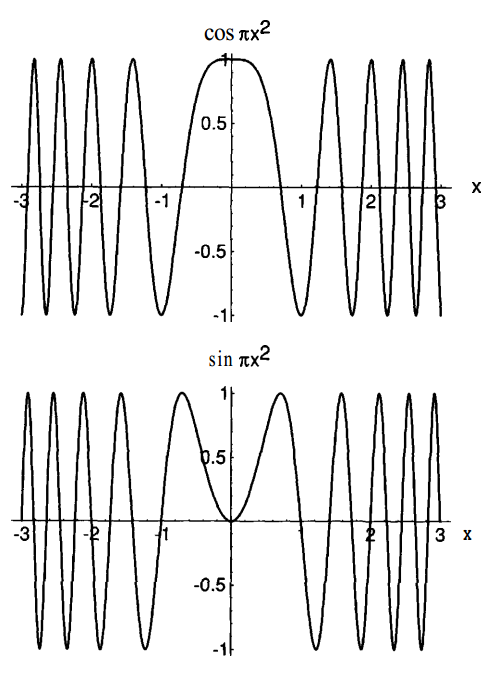
\includegraphics[scale=0.5]{../graphics/Wave_optics7.png}
	  \caption{Quadratic phase cosine and sine functions}
	  \label{fig:Quadratic}
	\end{figure}

	Figure \ref{fig:Quadratic} shows plots of one-dimensional quadratic-phase cosine and sine functions $\cos(\pi x^2)$ and $\sin(\pi x^2)$, each of them has the area of $1/\sqrt{2}$. Using this fact it can be shown that all of the unit area under the two-dimensional quadratic-phase exponential is contributed by the two-dimensional sinusoidal term.

	\begin{figure}[h!]
	  \centering
	  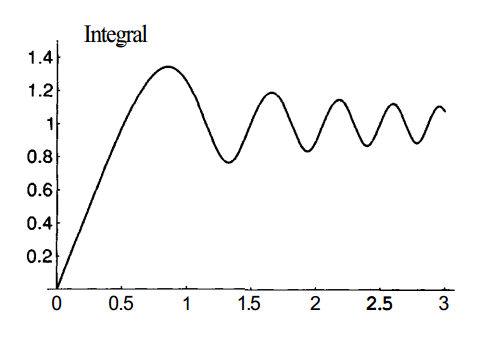
\includegraphics[scale=0.5]{../graphics/Wave_optics8.png}
	  \caption{Magnitude of the integral of the quadratic-phase exponential function}
	  \label{fig:Magnitude}
	\end{figure}

	Figure \ref{fig:Magnitude} shows the magnitude of the integral of a quadratic-phase exponential function
	\begin{equation}
	\abs{\int^X_{-X}{exp(j\pi x^2)dx}}=\abs{\sqrt{2}C(\sqrt{2}X)+j\sqrt{2}S(\sqrt{2}X)}
	\end{equation}
	which has also been expressed in terms of the Fresnel integrals C(z) and S(z) as
	\begin{align}
	C(z)=\int_0^z{\cos(\frac{\pi t^2}{2})}dt\\
	S(z)=\int_0^z{\sin(\frac{\pi t^2}{2})}dt
	\end{align}
	As can be seen from the figure, the integral grows towards its asymptotic value of unity with increaseing X. Note in particular the integral first reaches unity when X=0.5, and then oscillates about value with diminishing fluctuations. We conclude that, to a reasonable approximation, the major contributions to a convolution of this function with a second function that is smooth and slowly varying will come from the range $-2<X<2$, due to the fact that outside this range the rapid oscillations of the integrand do not yield a significant addition to the total arrea.

	For the scaled quadratic-phase exponential of \ref{Fresnel2}, the corresponding conclusion is that the majority of the contribution to the convolution integral comes from a square in the $(\xi,\eta)$ plane
	\begin{equation}
	-2<\frac{x}{\sqrt{\lambda z}}<2
	\end{equation}
	with the width $4\sqrt{\lambda z}$ and centered on the point $(\xi=x,\eta=y)$. This square grows in size as the distance z behind the aperture increases. In effect, when this square lies entirely within the open portion of the aperture, the field observed at distance z is, to a good approximation, what it would be if the aperture were not present. When the square lies entirely behind the obstruction of the aperture, then the observation point lies in a region that is, to a good approximation, dark due to the shadow of the aperture. When the square bridges the open and obstructed parts of the aperture, then the observed field is in the transition region between light and dark.
	\begin{figure}[h!]
	  \centering
	  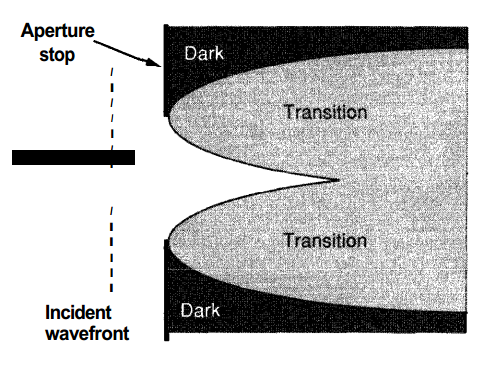
\includegraphics[scale=0.5]{../graphics/Wave_optics9.png}
	  \caption{Light, dark, and transition regions behind a rectangular slit aperture}
	  \label{fig:regions}
	\end{figure}
	Figure \ref{fig:regions} shows the case of a one-dimensional rectangular slit. The boundaries between the light region and the transition region, and between the dark region and the transition region can be shown to be parabolas.

	The idea is valid when the diffracting aperture do not contain fine structure and when they are illuminated by uniform plane waves. For the case when this conclusion may not hold, if the amplitude of the field transmitted by the aperture has a high-spatial-frequency sinusoidal component, that component may intract with the high frequencies of the quadratic-phase exponential kernel to produce a nonzero contribution from a location other than the square of $4\sqrt{\lambda z}$ mentioned above.

	When the distance z is allowed to approach zero,  i.e. the observation point approaches the diffracting aperture, then the two-dimensional quadratic-phase function behaves in the limit like a delta function,  roducing a field $U(x,y)$ that is identical to the aperture field $U(\xi,\eta)$in the aperture. In such a case, the predictions of geometrical optics are valid.

	Our discussion above is closely related to the principle of stationary phase, a method for finding the asymptotic values of certain integrals. The code PHASE uses stationary phase to calculate the integrand.
	\subsection{Fraunhofer Diffraction}
	Here we consider another more stringent approximation which, when valid, greatly simplifies the calculations. Continue from the equation \ref{Fourierform}, the observed field strength $U(x,y)$ can be found from a Fourier transform of the product of the aperture distribution $U(\xi,\eta)$ and a quadratic phase function $exp[j(k/2z)(\xi^2+\eta^2)]$. If the Fraunhofer approximation is satisfied:
	\begin{equation}
	z\gg \frac{k(\xi^2+\eta^2)_{max}}{2}
	\end{equation}
	Then the quadratic phase function $exp[j(k/2z)(\xi^2+\eta^2)]$ can be approximated as unity over the entire aperture, and the observed field strength can be found directly from a Fourier transform of the aperture distribution itself.Thus in the region of Fraunhofer diffraction or in the far field,
	\begin{equation}
	U(x,y)=\frac{exp(jkz)}{j\lambda z}exp\left[\frac{jk}{2z}(x^2+y^2)\right]\iint_{-\infty}^{+\infty} U(\xi,\eta)exp\left[-j\frac{2\pi}{\lambda z}(x\xi+y\eta)\right]d\xi d\eta\label{Fraunhofer}
	\end{equation}

	An alternative, less stringent condition, known as the "antenna designer's formula", states that for an aperture of linear dimension D, the Fraunhofer approximation will be valid provided
	\begin{equation}
	z>\frac{2D^2}{\lambda}
	\end{equation}

	\subsection{Fraunhofer diffraction for thin lens model(mirror)}

	\section{Wavefront propagation code}
	\subsection{ShadowOui}
	The hybrid method simulate the geometric effects of the optical components (mirror figures) and apertures by means of ray-tracing, whereas their diffraction contribution s are calculated independently for each element using wavefront propagation. The results from the diffraction contribution is integrated into the ray-tracing results by numerical convolution and ray re-sampling.
	\begin{enumerate}
	\item Ray-tracing traces the rays from source or continuation plane, through the optical element, and ends at the exit plane placed at zero distance downstream from the element. The rays are trimmed by effective aperture of element. This step takes into account the mirror figures and generates the corresponding ray divergences (dx,dz).
	\item Calculate the additional deviation of ray divergences by diffraction effect from the aperture or finite mirror size and from the figure errors. Propagate a plane wave through an element using Fourier optics methods.
	\item Convolute the beam divergences of ray-tracing and diffraction. It is based on the far-field approximation that the partially coherent beam incident on the optics can be viewed as a composition of plane waves with different propagation directions corresponding to the divergence distribution of geometric rays. Along each ray propagation direction, the plane wave diffracs through the optics and forms an angular distribution centered along that direction. The convolution of beam divergences at theexit plane of the optics is equivalent to the convolution of beam profiles due to ray-tracing and wavefront propagation at the image plane.
	\end{enumerate}
	Here we illustrate more on mathematical derivation.

	In case of an aperture, the electric field in the coordinates of the exit plane (x,z) is expressed as
	\begin{equation}
	E_e(x,z)=[I_{ray}(x,z)]^{1/2}
	\end{equation}
	where the phase of the plane wave is chosen to be zero for simplicity. The amplitude of the wave is determined from the intensity distribution $I_{ray}(x,z)$ given by the ray-tracing in the range of effective aperture dimension which is also obtained from ray-tracing.

	This equation can also apply to ideal mirror because the intensity distribution $I_{ray}$ is not only apertured but also modified by the focusing or defocusing condition of the element.

	For mirror with figure errors, we need to project the figure error profile from mirror coordinates $\Delta h(l,m)$ to $\Delta h(x,z)$, which introduces the phase shift
	\begin{equation}
	\Delta \phi_h(x,z)=-2k\Delta h(x,z)\sin\theta(x,z)
	\end{equation}
	where $k=2\pi/\lambda$ is the wave number. So the electric field at the exit plane becomes
	\begin{equation}
	E_e(x,z)=[I_{ray}(x,z)]^{1/2}exp[-2k\Delta h(x,z)\sin\theta(x,z)]
	\end{equation}
	with the specific effective aperture size calculated by ray-tracing.

	Then according to equation \ref{Fraunhofer} using Fraunhofer diffraction approximation, electric field at image plane is given by
	\begin{equation}
	E_i(x',z')=\frac{1}{j\lambda y}exp\left[\frac{jk}{2y}(x^2+z^2)\right]\iint_{-\infty}^{+\infty} E_e(x,z)exp\left[-\frac{jk}{z}(xx'+zz')\right]dxdz
	\end{equation}
	Then we can get the angle intensity profile, or angle probability distribution function, at the exit plane is then given by
	\begin{equation}
	I_e[\tan(dx),\tan(dz)]=\frac{I_i(x',z')}{y}=\frac{E_i(x',z')E_i^*(x',z')}{y}\label{angle distribution}
	\end{equation}

	The last two equations use Fraunhofer approximation and need to be noticed that $y\gg \Delta^2/\lambda$.

	The next step is to convolute the angle distribution from the wavefront propagation with the beam divergence from the ray-tracing at the exit plane of the optics. The convolution is achieved by re-sampling the divergences of all rays. For each ray, a random angle shift is generated based on the probability distribution function \ref{angle distribution} and added to the divergence value retained from the ray-tracing. The summed divergence value is then used to obtain the direction cosines of the new ray.

	Reviews on this algorithm:

	\begin{itemize}
	\item Even though this approximate approach was demonstrated to give correct results in some special cases of beamlines (e.g. with one secondary source aperture), it has, from our point of view, several important weaknesses, such as a necessity to make assumptions about radiation phase when extrapolating it from intensity, and a strongly increasing numerical complexity of the simulation when effects of diffraction at a number of apertures along the beam path have to be taken into account, in particular in a 2D simulation case.\\From Chubar, Oleg; Rakitin, Maksim S.; Chen-Wiegart, Yu-Chen; Chu, Yong S.; Fluerasu, Andrei; Hidas, Dean; Wiegart, Lutz (2017): Main functions, recent updates, and applications of Synchrotron Radiation Workshop code. In Kawal Sawhney, Oleg Chubar (Eds.): Advances in Computational Methods for X-Ray Optics IV. Advances in Computational Methods for X-Ray Optics IV. San Diego, United States, 6/8/2017 - 10/8/2017: SPIE, p. 5. Available online at https://www.spiedigitallibrary.org/conference-proceedings-of-spie/10388/2274285/Main-functions-recent-updates-and-applications-of-Synchrotron-Radiation-Workshop/10.1117/12.2274285.full.
	\item 
	\end{itemize}

	\subsection{SRW}

	\subsection{PHASE}

	\subsection{XRT}

	\subsection{WISE}

	\section{Other optical simulator}
	\subsection{ZEMAX OpticStudio}


	\section{Reference}
	\begin{itemize}
	\item Introduction to Fourier Optics 2ed Goodman J.W
	\item Shi, Xianbo; Reininger, Ruben; Sanchez Del Rio, Manuel; Assoufid, Lahsen (2014): A hybrid method for X-ray optics simulation. Combining geometric ray-tracing and wavefront propagation. In Journal of synchrotron radiation 21 (Pt 4), pp. 669–678. DOI: 10.1107/S160057751400650X.
	\end{itemize}

	\begin{equation}
	\beta'=\delta y'/\delta y
	\end{equation}
	\begin{table}[h!]
	\centering
	\caption{DABAM}
	\label{my-label}
	\begin{tabular}{lllll}
	\textbf{Entry} & \textbf{shape} & \textbf{Length[mm]} & \textbf{slp err [urad]} & \textbf{hgt err [um]}\\
	\hline
	1 & plane & 1200 & 0.49  (0.49 ) & 43.85  (43.85 ) \\
	2 & plane & 360 & 0.15  (0.15 ) & 4.46  (4.46 ) \\
	3 & spherical & 118 & 0.17  (0.17 ) & 1.56  (1.56 ) \\
	4 & elliptical & 32 & 0.13  (0.13 ) & 0.22  (0.22 ) \\
	5 & spherical & 429 & 0.84  (0.84 ) & 31.89  (31.90 ) \\
	6 & elliptical & 200 & 1.01  (1.01 ) & 2.98  (2.98 ) \\
	7 & plane & 99 & 0.58  (0.57 ) & 0.57  (0.51 ) \\
	8 & plane & 97 & 0.57  (0.57 ,0.67) & 4.05  (4.05 ,0.28) \\
	9 & plane & 97 & 0.44  (0.44 ,0.61) & 3.53  (3.52 ,0.41) \\
	10 & plane & 442 & 0.23  (0.23 ,0.23) & 6.20  (6.20 ,3.05) \\
	11 & plane & 445 & 0.23  (0.23 ,0.23) & 6.58  (6.59 ,3.23) \\
	12 & plane & 442 & 0.32  (0.32 ,0.32) & 2.93  (2.86 ,2.51) \\
	13 & spherical & 114 & 1.30  (1.29 ,1.51) & 9.11  (8.97 ,10.86) \\
	14 & spherical & 240 & 1.15  (1.14 ,1.05) & 23.38  (23.28 ,15.37) \\
	15 & toroidal & 800 & 2.13  (2.13 ,2.13) & 170.87  (170.87 ,97.36) \\
	16 & toroidal & 239 & 1.85  (1.84 ,1.86) & 54.67  (54.78 ,36.54) \\
	17 & toroidal & 495 & 2.27  (2.27 ,2.40) & 61.49  (61.54 ,47.58) \\
	18 & cylindrical & 330 & 0.12  (0.12 ,0.12) & 1.83  (1.83 ) \\
	19 & elliptical & 350 & 0.14  (0.14 ,0.06) & 7.25  (7.25 ) \\
	20 & elliptical & 121 & 0.45  (0.45 ,0.50) & 3.40  (3.40 ) \\
	21 & elliptical & 430 & 0.43  (0.43 ,0.50) & 6.05  (6.05 ) \\
	22 & cylindrical & 1130 & 5.32  (5.32 ,5.00) & 400.83  (400.82 ) \\
	23 & plane & 127 & 0.18  (0.18 ,0.18) & 2.17  (2.17 ) \\
	24 & plane & 774 & 0.20  (0.20 ,0.20) & 5.35  (5.35 ) \\
	25 & plane & 200 & 0.07  (0.07 ,0.07) & 1.48  (1.47 ,1.33) \\
	26 & spherical & 948 & 0.86  (0.86 ) & 94.47  (94.52 ) \\
	27 & Toroidal & 289 & 1.86  (1.85 ,1.80) & 41.98  (41.98 ) \\
	28 & Plane & 439 & 0.95  (0.95 ,0.93) & 51.74  (51.73 ) \\
	\end{tabular}
	\end{table}
	\begin{table}[h!]
	\centering
	\caption{DABAM}
	\label{my-label}
	\begin{tabular}{lllll}
	\textbf{Entry} & \textbf{shape} & \textbf{Length[mm]} & \textbf{slp err [urad]} & \textbf{hgt err [um]}\\
	\hline
	29 & Spherical & 185 & 0.60  (0.60 ,0.55) & 5.22  (5.22 ) \\
	30 & Plane & 480 & 0.89  (0.89 ) & 37.01  (37.00 ) \\
	31 & Plane & 299 & 0.56  (0.56 ) & 14.93  (14.93 ) \\
	32 & Plane & 299 & 1.33  (1.33 ) & 61.19  (61.28 ) \\
	33 & Plane & 390 & 0.29  (0.29 ) & 6.81  (6.80 ) \\
	34 & Plane & 239 & 0.44  (0.44 ) & 11.64  (11.66 ) \\
	35 & Plane & 239 & 0.45  (0.45 ) & 6.95  (6.93 ) \\
	36 & Plane & 239 & 0.48  (0.48 ) & 7.75  (7.74 ) \\
	37 & Spherical & 1000 & 0.32  (0.32 ) & 11.95  (11.95 ) \\
	38 & Spherical & 1000 & 0.53  (0.53 ) & 45.00  (44.99 ) \\
	39 & Elliptical(Unbent) & 1000 & 0.34  (0.34 ) & 20.41  (20.41 ) \\
	40 & Elliptical(Unbent) & 1000 & 0.35  (0.35 ) & 22.64  (22.64 ) \\
	41 & Spherical & 700 & 0.44  (0.44 ,0.00) & 16.35  (16.34 ,0.00) \\
	42 & Elliptical(Detrended) & 900 & 1.78  (1.78 ) & 174.91  (174.91 ) \\
	43 & Toroid(Unbent) & 598 & 0.92  (0.92 ) & 16.98  (16.99 ) \\
	44 & Toroid(Unbent) & 598 & 1.95  (1.95 ) & 25.97  (25.98 ) \\
	45 & toroidal & 1300 & 0.78  (0.78 ,0.78) & 101.37  (101.37 ,62.00) \\
	46 & toroidal & 1300 & 0.75  (0.75 ,0.75) & 89.86  (89.86 ,55.00) \\
	47 & toroidal & 1300 & 0.86  (0.86 ,0.86) & 101.70  (101.70 ,64.00) \\
	48 & toroidal & 1200 & 0.80  (0.80 ,0.80) & 80.45  (80.45 ,34.00) \\
	49 & toroidal & 1200 & 1.50  (1.50 ,1.47) & 186.95  (186.95 ,130.00) \\
	50 & toroidal & 1200 & 0.49  (0.49 ,0.49) & 34.44  (34.44 ,27.00) \\
	51 & plane & 190 & 0.38  (0.38 ,0.40) & 8.15  (8.14 ,5.50) \\
	52 & plane & 190 & 0.61  (0.61 ,0.60) & 10.11  (10.09 ,5.50) \\
	53 & plane & 140 & 0.34  (0.33 ,0.33) & 5.42  (5.41 ,3.00) \\
	54 & plane & 140 & 0.38  (0.38 ,0.38) & 4.28  (4.25 ,2.10) \\
	55 & Toroid(Unbent) & 900 & 1.60  (1.60 ) & 153.46  (153.30 ) \\
	56 & Toroid(Unbent) & 600 & 0.53  (0.53 ) & 18.16  (18.15 ) \\
	\end{tabular}
	\end{table}
\end{document}